\section{Task III : Predicting First Medal Countries}
\subsection{Problem Analysis}

More than 60 countries have still yet to win an Olympic medal.

We are required to predict how many countries will win their first medal in the 2028 Los Angeles Olympics, their probability of winning a medal, and their winning rate compared to each other.
\subsection{Model Establishment}

To establish the model( Codes are in the appendix ):

Firstly,we filter out those countries that won medals in 1896.Then we create a feature set for each country, encode the country name, and use the countries' first medal winning data splited as the training set and testing set to train the model using Random Forest Classifier.
Secondly, we predict the probability of `no medal'country winning a medal in the 2028 Los Angeles Olympics.
Finally, we calculate the winning rate of those country and compare them.

The basic rules of the Random Forest model are as follows:

$$\hat{y} = \frac{1}{N} \sum_{i=1}^{N} f_i(x)$$

where $N$ is the number of trees, and $f_i(x)$ is the result of each tree.

Each tree is built using a random subset of the data and features, which helps in reducing overfitting and improving generalization. The final prediction is obtained by averaging the predictions of all individual trees.

Next, we use a series of splits to decide the output:

$$f(x_i) =  
    y_i, \text{if } x \in \text{leaf}_i \\ 
$$

where $x$ is the feature vector, $\text{leaf}_i$ is the $i$th node, and $y_i$ is the prediction of node $i$.

The importance of each feature can be evaluated by measuring the decrease in impurity (e.g., Gini impurity or entropy) for each feature split across all trees:

$$\text{I}_{f}(j) = \sum_{t=1}^{N} \sum_{s \in \text{splits}(t)} \Delta \text{I}_{m}(s,j)  $$

where $\Delta$ stands for decrease and $\text{splits}(t)$ are the splits in tree $t$.

\subsection{Result Analysis}
\begin{center}
    $N_u$ = 79
\end{center}

This value may be slightly more than the real number of countries that have not won a medal, as some countries which didn't win a medal in the past may have vanished from the earth due to historical or political reasons, and some countries may be the same country but have different country names which are not detected by the `country map' preprocession. However, the calculation is rather accurate. From the information on the internet, there are more than 60 or 70 countries that have not won a medal in the Olympics.

If we assume that a probability of winning a medal greater than 0.3 is a good chance of winning a medal, then 7 countries have a good chance of winning a medal in the 2028 Los Angeles Olympics.The definition of good chance varies from person to person, and the threshold can be adjusted according to the actual situation. A probability distribution histogram is also provided in \textbf{Figure \ref{fig:win_probability_distribution}} , which can indicate some interesting factors.


\begin{figure}[h]
    \centering
    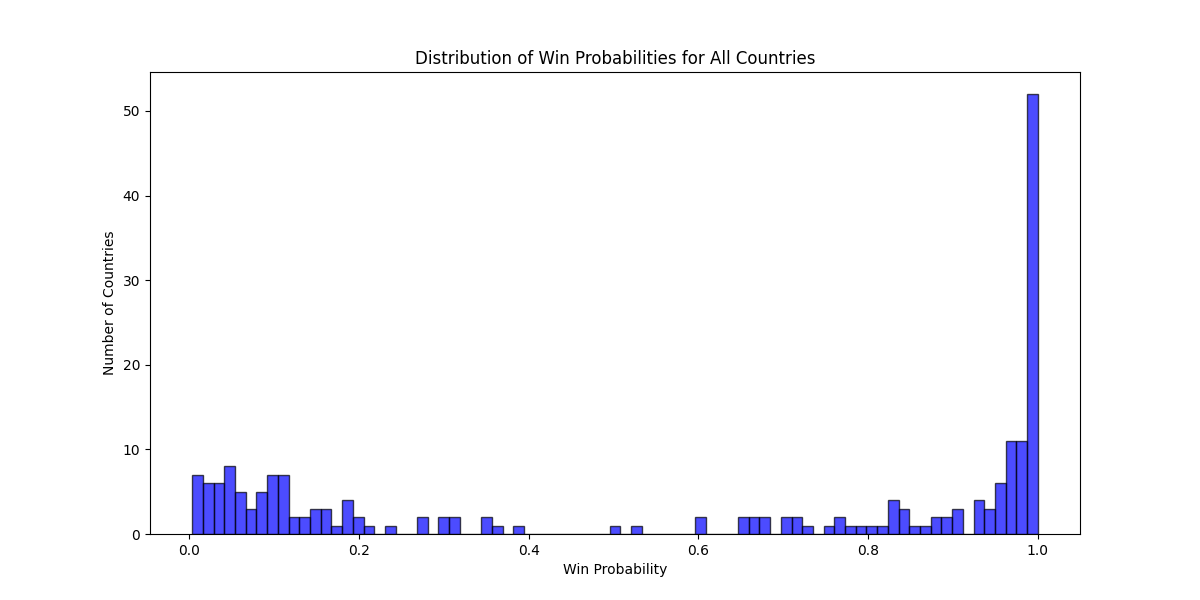
\includegraphics[width=0.8\textwidth]{../figures/win_probability_distribution.png}
    \caption{Distribution of Win Probabilities for All Countries}
    \label{fig:win_probability_distribution}
\end{figure}

The winning probability of those countries shows a distribution trend of the opposite of gaussian distribution : countries with low and high probability are more than countries with medium probability, and the trend is like a curve which is low in the middle and high at both ends, and the winning probability of some countries is extremely high. That can be explained in real world, as countries which have not got a medal are more likely to be new countries participating in the Olympics or countries that have attended a lot with still no medal, which is very likely to win a medal in the future. Most of the countries attending the Olympics are easy to win over than one medal, and there are still some countries struggling to win.
\begin{figure}[h]
    \centering
    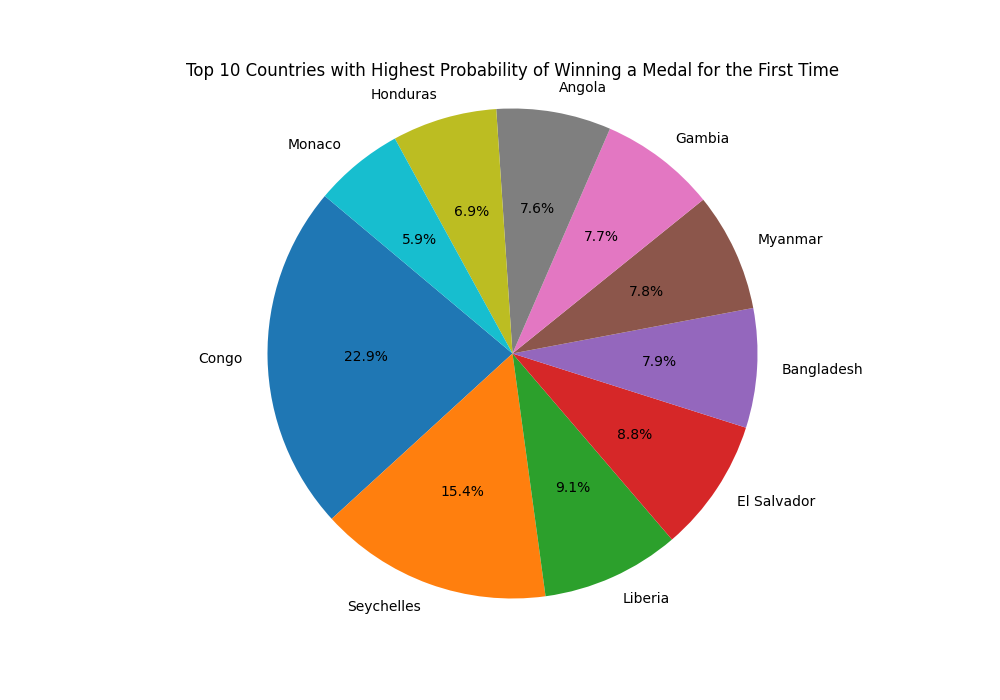
\includegraphics[width=0.8\textwidth]{../figures/first_medal_pie.png}
    \caption{First Medal Results}
    \label{fig:first_medal_pie}
\end{figure}

We've also drawn a pie chart to show the winning odds of top $10$ countries in \textbf{Figure \ref{fig:first_medal_pie}}. 

Congo has a extremely high winning probability of $90.28\%$ , while Liberia has a decent winning probability of $35.97\%$. Those two countries are typical African countries which have long strived to win a medal but failed due to various reasons. We sincerely hope that they will get their first medal in the 2028 Los Angeles Olympics.